{\fontsize{12pt}{22pt} \textbf{SMOTE}\par}

\vspace{5mm}

SMOTE is an oversampling method to generate data by drawing a distance between a point and a random neighbor. It is used to grow the size of a minority class. \\

\textit{Note}: the first part (until line 6) is the algorithm preliminaries. It allows to define what part of the minority class is going to be used for the new data generation.

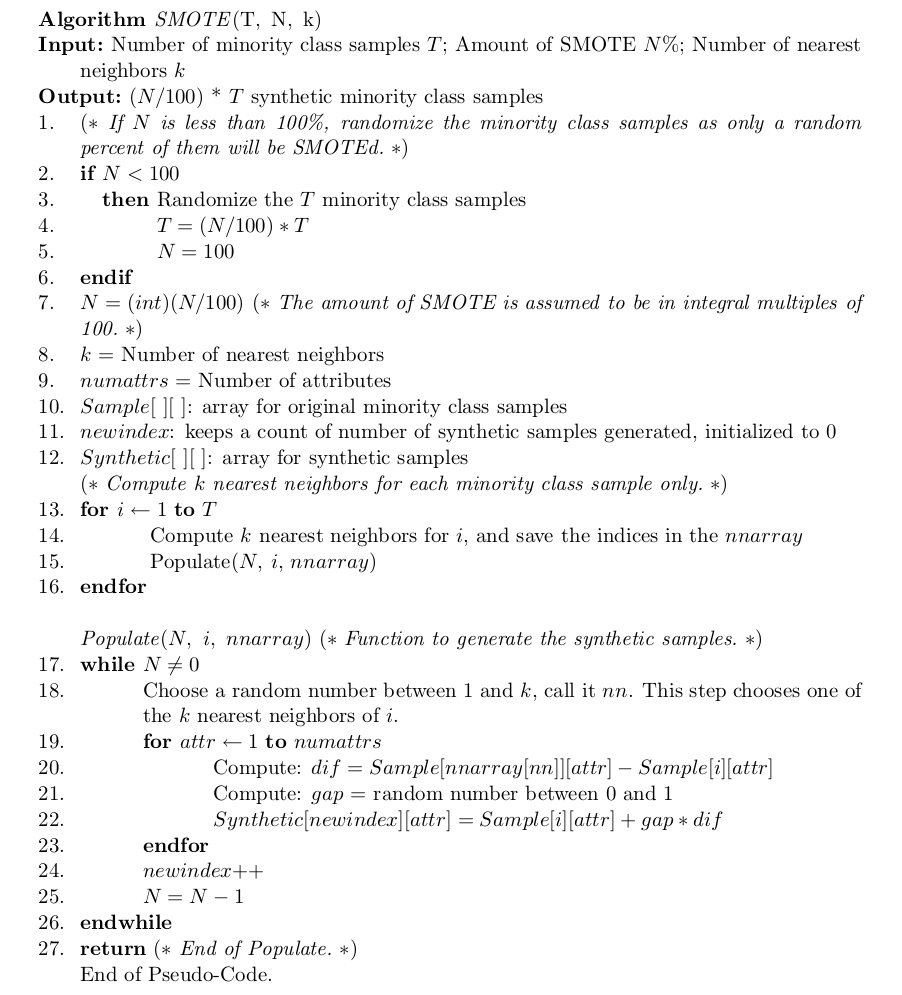
\includegraphics[scale=0.4]{SMOTE_algo.png}

\begin{algorithm}
\caption{SMOTE (simplified)}
\begin{algorithmic}
\For{$sample$ in $all\_samples$}
\State Choose a random neighbor 
\For{$attribute$ in $all\_attributes$}
\State Compute a random weighted distance between $sample$ attribute and $k$ attribute
\State Assign this distance to the newly generated point
\EndFor
\EndFor
\end{algorithmic}
\end{algorithm}

\begin{center}
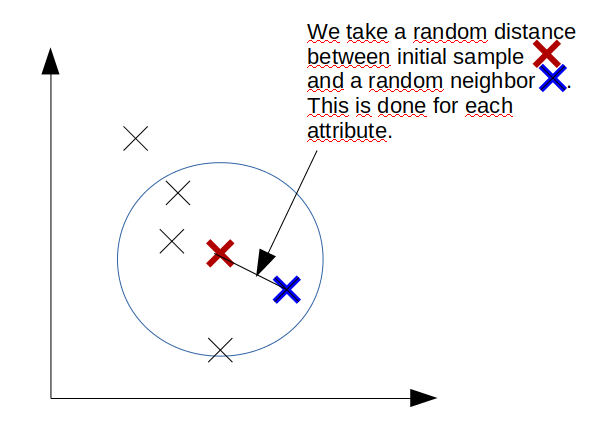
\includegraphics[scale=0.4]{SMOTE_schema.png}
\end{center}

\vspace{5mm}